\subsubsection{Cerca en Amplada (BFS)}

La cerca en amplada (breadth-first search) és molt semblant a la cerca en profunditat, però aquesta visita els nodes en ordre creixent a la seva distància des del node inicial. Així podem calcular molt fàcilment la distància des del node inicial fins a la resta de nodes, tanmateix, la cerca en amplada generalment és una mica més difícil d'implementar que la cerca en profunditat.

La cerca en amplada passa primer per tots els nodes els quals estan a una distància 1 del node inicial, és a dir que estan separats per una aresta, després pels que estan a una distància 2 i així successivament fins que tots els nodes ja han estat visitats.

\begin{center}
    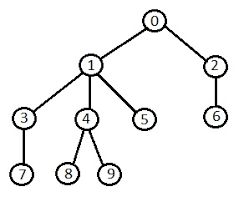
\includegraphics[width=.4 \textwidth]{TreeRoot.png}
    
    \caption{\emph{Figura 14: Graf (arbre). Font: \url{https://www.chegg.com/homework-help/questions-and-answers/consider-tree-tfe1png-answer-following-1-tis-rooted-vertex-2-siblings-vertex-3-3-parent-ve-q54883116}}}
\end{center}

Per exemple donat el graf de la figura 14, suposem que es pren com a node inicial el 0, llavors primerament visitem tots els nodes que estan a distància 1 del node 0, és a dir, visitem els nodes [1, 2], seguidament visitem els nodes [3, 4, 5, 6] i finalment visitem els nodes [7, 8, 9, 10].

Igual que la cerca en profunditat, la cerca en amplada té una complexitat temporal de $O(n + m)$, on $n$ és el nombre de nodes i $m$ el nombre d'arestes. \newline

En la següent implementació de l'algorisme BFS, recorrem tots els nodes que podem assolir des d'un node inicial a la vegada que ens guardem la distància a la qual estan tots els nodes del node inicial en un graf connex i no dirigit. \newpage


\begin{lstlisting}
vector<vector<int>> adjacents;  // Aquí guardem el graf
vector<bool> visitats;          // Aquí guardem els nodes visitats
vector<int> dist;               // Aquí guardem les distàncies

void BFS(){
    queue<int> cua;
    cua.push(1);   // Prenem el node 1 com a inicial    
    dist[1] = 0;   // Marquem distància 0 al node inicial
    
    while (!cua.empty()){ // Mentre que puguem visitar nodes
        int node = cua.front(); // Agafem el node del principi de la cua
        cua.pop();  // Traiem el node de la cua
        visitats[node] = 1; // Marquem el node com a visitat
        for (auto nodeAdjacent : adjacents[node]){ // Mirem nodes adjacents
            if (visitats[nodeAdjacent] == false){ // Si no l'hem visitat
                cua.push(nodeAdjacent);  // L'afegim a la cua
                dist[nodeAdjacent] = dist[node] + 1; 
                // La distància és igual a la del node del qual venim + 1
            }
        }
    }
}

int main(){ 
    BFS();  

    for (int i = 0; i < n; i++)
        if (visitats[i] == true)
            cout << dist[i] << " "; 
            // Imprimim les distàncies dels nodes visitats
}
\end{lstlisting}


L'algorisme BFS sempre visita els nodes per ordre de distància des del node inicial gràcies a l'estructura de dades cua, ja que com que els nodes s'afegeixen al final de la cua i s'agafen del principi de la cua, no es seguirà un camí definit sinó que la cerca es realitza en amplada.

Per entendre-ho millor, amb el següent graf, faré una representació de com actuaria el BFS en aquest cas, en cada pas mostraré com seria la cua (la dreta representa el principi de la cua) i com seria el vector distàncies. \newpage



\begin{center}
    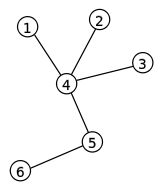
\includegraphics[width=.4 \textwidth]{tree.png}
    
    \caption{\emph{Figura 15: Graf (arbre). Font: \url{https://en.wikipedia.org/wiki/Tree_(graph_theory)}}}
\end{center}



Començarem per exemple pel node 1, l’afegim al final de la cua i li donem valor 0 a la distància. \newline

\textbf{Cua} [1]

\textbf{Dist} [1 : 0] \newline

Traiem el node 1 de la cua, mirem els nodes adjacents el node 1, afegim al final de la cua el node 4. \newline

\textbf{Cua} [4]

\textbf{Dist} [1 : 0] \newline

Traiem el node 4 de la cua, li donem valor 1 a la distància, mirem els seus nodes adjacents, afegim els nodes 2,3 i 5 al final de la cua. \newline

\textbf{Cua} [2, 3, 5]

\textbf{Dist} [1 : 0, 4 : 1] \newline

Traiem el node 5 de la cua, li donem valor 2 a la distància, mirem els seus nodes adjacents, afegim el node 6 al final de la cua. \newline

\textbf{Cua} [6, 2, 3]

\textbf{Dist} [1 : 0, 4 : 1, 5 : 2] \newline

Traiem el node 3 de la cua, li donem valor 2 a la distància, mirem els seus nodes adjacents, no afegim cap node a la cua, ja que el seu node adjacent (4) ja ha estat visitat. \newline

\textbf{Cua} [6, 2]

\textbf{Dist} [1 : 0, 3 : 2, 4 : 1, 5 : 2] \newline

Traiem el node 2 de la cua, li donem valor 2 a la distància, mirem els seus nodes adjacents, no afegim cap node a la cua puix que el seu node adjacent (4) ja ha estat visitat. \newline

\textbf{Cua} [6]

\textbf{Dist} [1 : 0, 2 : 2, 3 : 2, 4 : 1, 5 : 2] \newline

Traiem el node 6 de la cua, li donem valor 3 a la distància, mirem els seus nodes adjacents, no afegim cap node a la cua, ja que el seu node adjacent (5) ja ha estat visitat. \newline

\textbf{Cua} []

\textbf{Dist} [1 : 0, 2 : 2, 3 : 2, 4 : 1, 5 : 2, 6 : 3] \newline

Com que la cua està buida, vol dir que ja hem visitat tots els nodes que podíem visitar i, per tant, el BFS finalitza.


